\documentclass[a4paper,14pt]{extreport}
  \usepackage[left=1.5cm,right=1.5cm,
      top=1.5cm,bottom=2cm,bindingoffset=0cm]{geometry}
  \usepackage{scrextend}
  \usepackage[T1,T2A]{fontenc}
  \usepackage[utf8]{inputenc}
  \usepackage[english,russian,ukrainian]{babel}
  \usepackage{tabularx}
  \linespread{1.3}
  \usepackage[colorinlistoftodos]{todonotes}
  \usepackage{amssymb}
  \usepackage{color}
  \usepackage{amsmath}
  \usepackage{mathrsfs}
  \usepackage{listings}
  \usepackage{graphicx}
  \graphicspath{ {./images/} }
  \usepackage{lipsum}
  \usepackage{xcolor}
  \usepackage{hyperref}
  \usepackage{tcolorbox}

  \usepackage[framemethod=TikZ]{mdframed}
  \usepackage{wrapfig,boxedminipage,lipsum}
  \mdfdefinestyle{MyFrame}{%
  linecolor=blue,outerlinewidth=2pt,roundcorner=20pt,innertopmargin=\baselineskip,innerbottommargin=\baselineskip,innerrightmargin=20pt,innerleftmargin=20pt,backgroundcolor=gray!50!white}
   \usepackage{csvsimple}
   \usepackage{supertabular}
  \usepackage{pdflscape}
  \usepackage{fancyvrb}
  %\usepackage{comment}
  \usepackage{array,tabularx}
  \usepackage{colortbl}

  \usepackage{varwidth}
  \tcbuselibrary{skins}
  \usepackage{fancybox}
  \usepackage{spreadtab}


  \usepackage{tikz}
  \usepackage[framemethod=TikZ]{mdframed}
  \usepackage{xcolor}
  \usetikzlibrary{calc}
  \makeatletter
  \newlength{\mylength}
  \xdef\CircleFactor{1.1}
  \setlength\mylength{\dimexpr\f@size pt}
  \newsavebox{\mybox}
  \newcommand*\circled[2][draw=blue]{\savebox\mybox{\vbox{\vphantom{WL1/}#1}}\setlength\mylength{\dimexpr\CircleFactor\dimexpr\ht\mybox+\dp\mybox\relax\relax}\tikzset{mystyle/.style={circle,#1,minimum height={\mylength}}}
  \tikz[baseline=(char.base)]
  \node[mystyle] (char) {#2};}
  \makeatother
   % Цвета для гиперссылок
  \definecolor{linkcolor}{rgb}{0, 0.72, 0.92} % цвет ссылок
  \definecolor{urlcolor}{rgb}{0.0, 0.0, 1.0}% цвет гиперссылок
  \hypersetup{pdfstartview=FitH,  linkcolor=red,urlcolor=red,citecolor=red, colorlinks=true}

  \definecolor{ggreen}{rgb}{0.4,1,0}
  \definecolor{rred}{rgb}{1,0.1,0.1}
  \definecolor{amber}{rgb}{1.0, 0.75, 0.0}
  \definecolor{babyblue}{rgb}{0.54, 0.81, 0.94}
  \definecolor{amethyst}{rgb}{0.6, 0.4, 0.8}

  \usepackage{float}
  \usepackage{wrapfig}
  \usepackage{framed}
  %for nice Code{
  \lstdefinestyle{customc}{
    belowcaptionskip=1\baselineskip,
    breaklines=true,
    frame=L,
    xleftmargin=\parindent,
    language=C,
    showstringspaces=false,
    basicstyle=\small\ttfamily,
    keywordstyle=\bfseries\color{green!40!black},
    commentstyle=\itshape\color{purple!40!black},
    identifierstyle=\color{blue},
    stringstyle=\color{orange},
  }
  \lstset{escapechar=@,style=customc}
%}


\begin{document}
\renewcommand{\bibname}{Список використаної літератури}% -- переименуем название списка литературы


%указатель -- \cite{lit1}

\pagecolor{white}

%----------------------------------------1
\newtcbox{\xmybox}[1][red]{on line, arc=7pt,colback=#1!10!white,colframe=#1!50!black, before upper={\rule[-3pt]{0pt}{10pt}},boxrule=1pt, boxsep=0pt,left=6pt,right=6pt,top=2pt,bottom=2pt}

\begin{titlepage}
  \begin{center}
  \large
  Національний технічний університет України \\ "Київський політехнічний інститут імені Ігоря Сікорського"


  Факультет Електроніки

  Кафедра мікроелектроніки
  \vfill

  \textsc{РЕФЕРАТ}\\

  %{\Large Про виконання лабораторної роботи №1\\
  з дисципліни: «Фізичні основи сенсорики»\\[1cm]

  Сенсори в роботехніці


  %}
  \bigskip
  \end{center}
  \vfill

  \newlength{\ML}
  \settowidth{\ML}{«\underline{\hspace{0.4cm}}» \underline{\hspace{2cm}}}
  \hfill
  \begin{minipage}{1\textwidth}
  Виконавець:\\
  Студент 4-го курсу \hspace{4cm} $\underset{\text{(підпис)}}{\underline{\hspace{0.2\textwidth}}}$  \hspace{1cm}Грабар О. О.\\
  \vspace{1cm}

  Перевірила: \hspace{5.6cm} $\underset{\text{(підпис)}}{\underline{\hspace{0.2\textwidth}}}$  \hspace{1cm} Коваль В. М.\\

  \end{minipage}

  \vfill

  \begin{center}
  2021
  \end{center}
\end{titlepage}
\tableofcontents
\setcounter{page}{2}

\newpage


  %\section{Подраздел}


%  \begin{figure}[h]
%   \center{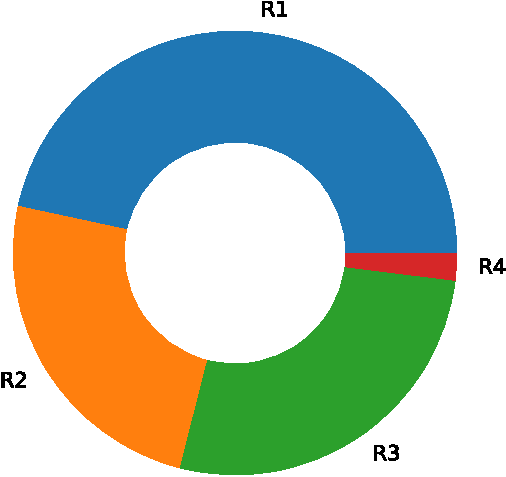
\includegraphics[width=0.9\linewidth]{2.jpg}}
%   \caption{Перший апарат магнітного запису.}
%   \label{ris2}
% \end{figure}
\chapter{Сенсори для роботів та їх характеристики.}
\section{Що таке сенсори для робототехніки?}\par

 Сенсори для робототехніки -- це датчики, які робот використовує для зв'язку з довкіллям, обчислюючи фізичні величини навколо себе. Датчики працюють на основі теорії трансдукції, яка включає перетворення енергії з однієї форми на іншу, а отримані дані обробляються контролером, що дозволяє роботу діяти. Датчики роботів також відстежують стан робота і навколишню ситуацію.\\

\begin{figure}[h!]
   \center{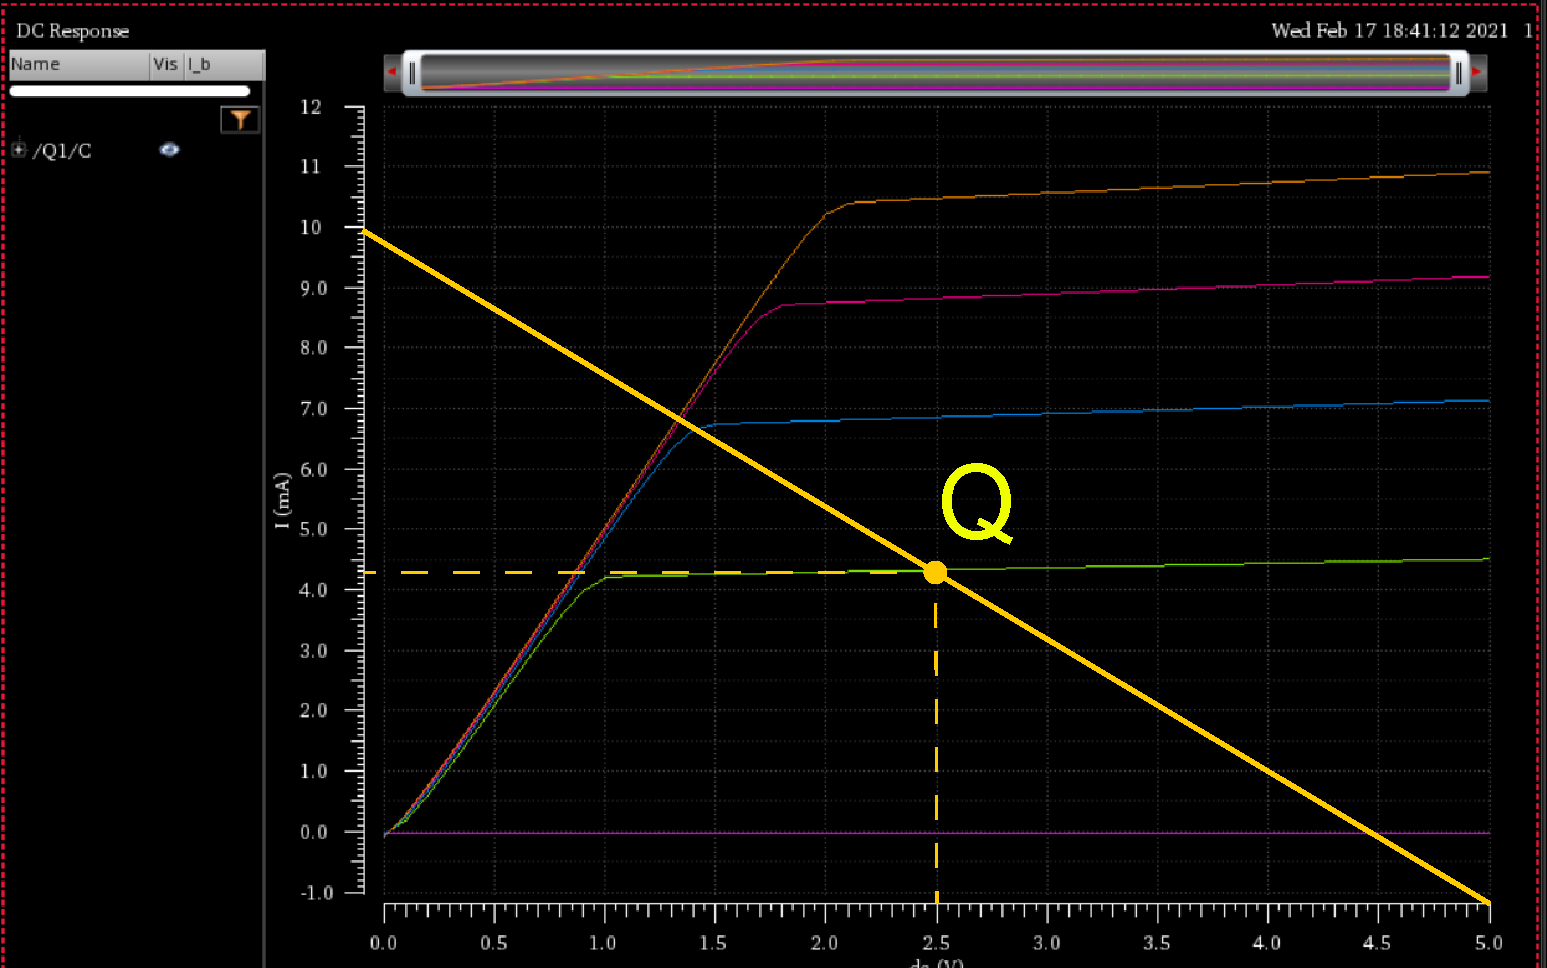
\includegraphics[width=0.8\linewidth]{1.png}}
   \caption{Різні типи датчиків роботів; Кредити зображень: Фонд робототехніки з відкритим вихідним кодом, Роботизовані датчики, CC BY 3.0}
 \end{figure}

   Як згадувалося раніше, датчики роботів використовуються для оцінки стану робота та його оточення. Щоб забезпечити прийнятну поведінку, сигнали передаються контролеру. Роботизовані сенсори змодельовані за ролями органів чуття людини. Для правильної роботи роботам необхідно багато знати про своє оточення.
 
\section{Чому рецептори важливі для роботів?}\par

Датчики роботів можуть бути механічними, хімічними або електричними за своєю природою, і робота кожного датчика заснована на принципі перетворення, що передає енергію від одного типу до іншого. Датчики робота дозволяють роботу гнучко реагувати на навколишнє оточення. Роботи можуть бачити і відчувати за допомогою датчиків, які дозволяють виконувати більш складні завдання.\\ 

Датчики роботів відстежують стан роботів та їхнє оточення, відправляючи електронні сигнали на контролери роботів. Датчики потрібні роботам, щоб контролювати себе. Роботам необхідні знання про місцезнаходження та рух їх тіл та частин, щоб контролювати їхню поведінку.

\section{Характеристики датчиків у робототехніці}\par

Характеристики датчиків робота допомагають нам визначити відповідний датчик для робота у різних ситуаціях. Деякі з основних атрибутів датчиків роботів описані нижче:

\subsection{Точність}
Точність датчика відноситься до близькості зареєстрованого значення датчика до фактичного значення. Це часто формулюється як діапазон значень. Наприклад, +/- 1 мм. Подивившись на розділ калібрування нижче, часто можемо підвищити точність датчиків робота. Отже, точність - це різниця між вихідним сигналом датчика і фактичним значенням, тобто похибка = виміряне значення - дійсне значення.

\subsection{Калібрівка}
Точність та дозвіл датчиків робота також можна підвищити шляхом їх калібрування. Окремий розділ присвячений дозволу. Калібрування - це метод порівняння характеристик датчика з деякими відомими величинами, який може бути виконаний продавцем або вами, і ця інформація може бути використана для створення рівняння, що зв'язує ці два параметри.\\

Це рівняння дасть кращі результати, ніж стандартні значення при обробці даних датчика. Ви також повинні розуміти, коли датчик стає перевантаженим (коли ви піднімаєтесь вище або нижче за межу того, що він може виміряти), і дані стають менш надійними або безглуздими.

\subsection{Дозвіл}
Дуже важливо знати, наскільки малу частину можуть виявити датчики робота, поки ми не дізнаємося, наскільки вона точна. Датчик температури з роздільною здатністю, наприклад, 5 градусів, наприклад, не може розрізнити 30 і 32 градуси. В результаті під роздільною здатністю розуміється найменша зміна вхідного сигналу, яку датчик може виявити та надійно вказати. Наприклад, який дозвіл у звичайної лінійки чи штангенциркуля?

\subsection{Лінійність}
Незалежно від того, є робота датчиків робота лінійною чи ні, ця інформація стає корисною при подачі вихідних даних датчика на низькорівневий комп'ютер, який не може виконувати багато обчислень і складати рівняння калібрування. Калібрувальна крива визначає лінійність. У статичних умовах фіксована еталонна крива відображає амплітуду o/p залежно від амплітуди i/p і має схожість із прямою лінією чи лінійністю.

\subsection{Повторюваність}
Важливою особливістю датчиків робота є те, що вони повинні давати однаковий результат щоразу, коли ви вимірюєте одні й самі умови. Це забезпечує повторюваність датчиків.

\subsection{Мертва зона та гістерезис}
У механічних системах, таких як роботи, деяка похибка в шестернях завжди викликає різне значення в залежності від напрямку руху (гістерезис) або зони нечутливості, коли датчики робота не виявляють будь-який рух.

\subsection{Дрейфувати}
Розрахунок конкретних датчиків робота має власний дрейф. Це особливо правильно для швидкісних гіроскопів. Вам знадобиться модель із низьким дрейфом (що менше дрейф, тим більше вона коштує), а також з можливістю фільтрації вихідного сигналу датчиків. Наприклад, робот нерухомий; Зрозуміло, що датчик не обертається, тому ви можете ігнорувати гіроскоп і робити незвичайні речі, наприклад, ігнорувати датчик і/або визначати швидкості дрейфу і застосовувати їх для підвищення продуктивності датчика.

\subsection{Температура}
Температура і двох компонентів, які визначають характеристики датчиків робота. Перше – це можливість підтримувати температурний режим. Поширена проблема з багатьма датчиками полягає в тому, дрейфує/змінюється значення датчика при зміні температури чи ні. Також є два розділи другої специфікації температури:\\
\begin{enumerate}
\item Корисна температура - Який мінімальний та максимальний діапазон температур датчика?
\item Температура зберігання - яка найнижча/найвища температура, за якої датчики можуть бути, поки вони не будуть пошкоджені?
\end{enumerate}

\begin{figure}[h!]
   \center{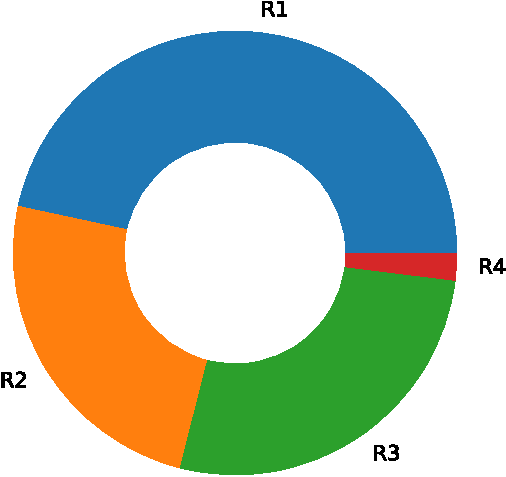
\includegraphics[width=0.8\linewidth]{2.png}}
   \caption{Датчики роботів: Датчик температури LM 35, Датчик температури LM35 напівпровідниковий термометр 1480374 5 6 HDR підсилювач, CC BY-SA 3.0}
 \end{figure}


\subsection{Поле зору (FOV)}
FOV (поле зору) – це важлива характеристика, яка вказує, яку область (зазвичай кутову) можуть бачити датчики робота. Часто згадуються горизонтальний (hFOV) та вертикальний (vFOV) компоненти. Наприклад, 70 × 30 градусів є hFOV x vFOV відповідно.

\subsection{Розмір плями}
В основному це стосується лазерів, але важливо знати, наскільки великий розмір плями на заданій відстані (пляма стає більшою зі збільшенням простору). Цей розмір плями має вирішальне значення визначення розміру видимих  предметів. Для перегляду крізь пил, дощ та сніг потрібен невеликий розмір плями. Щоб висловити це, можна використовувати як горизонтальну, і вертикальну шкалу плям. Виробники датчиків роботів зазвичай публікують лише одне із двох значень, тому що інше більше.

\subsection{Форма виходу}
Потрібно розуміти вихідну форму датчика. Наприклад, для аналогового виходу вам може знадобитися, який діапазон напруги або опору. Якщо виробництво перебуває на вищій стадії, переконайтеся, що у вас є відповідні вихідні дані. 4-20 мА, напруга, USB, Ethernet, послідовний порт і CAN – всі поширені типи виходів. Майте на увазі, що в камерах з гігабітним Ethernet часто використовується пакет jumbo (великий MTU), несумісний зі стандартами бездротового зв'язку 802.11 і потребує дротового з'єднання.

\subsection{Увімкнення}
Щоб правильно запитати систему, необхідно знати скільки енергії споживають датчики робота і який діапазон напруги вони можуть приймати. Деякі датчики роботів будуть мати широкий діапазон, в той час як іншим буде потрібно лише один DC-DC для строго контрольованого вхідного напруги.

\subsection{Надійність}
Надійність – це складний параметр для оцінки датчиків робота. На надійність впливають кілька чинників. Наскільки добре програма розроблена та надійна? Чи є датчик міцним з погляду фізичної міцності? Він добре збудований? Чи є електробезпека (захисні діоди, запобіжники тощо. буд.)? Рознімання в хорошому стані? Роз'єми випадуть? Він водостійкий? Чи є пиленепроникний ущільнювач? Список таких питань ніколи не може бути недостатнім.



\section{Як класифікуються датчики? | Типи датчиків роботів}\par

\subsection{Пропріоцептивні та екстероцептивні датчики в робототехніці}
Первинна класифікація датчиків робота проводиться на основі розташування стимулу.

\subsection{Пропріоцептивні датчики Внутрішні датчики у робототехніці}
Пропріоцептивні  рецептори дають роботу відчуття власної гідності. Вони обчислюють внутрішні характеристики роботизованої системи, такі як кут зчленування, положення коліс, рівень заряду батареї і т.д.

\subsection{Екстероцептивні датчики Зовнішні датчики у робототехніці}
Датчики, які надають інформацію про зовнішній стан, наприклад спостереження за довкіллям та його об'єктами, відомі як екстероцептивні.

\subsection{Активні та пасивні датчики в робототехніці}
Інший набір класифікації заснований на способі розсіювання енергії.

\subsection{Активні датчики у робототехніці}
Активні датчики, такі як датчики на основі радара, працюють шляхом випромінювання випромінювання (A).

\subsection{Пасивні датчики у робототехніці}
Пасивні датчики - це датчики, які пасивно одержують енергію, наприклад, камера.

 







\section{Як роботи використовують датчики? | Які проблеми можуть вирішити роботи за допомогою датчиків?}\par



\subsection{Застосування датчиків у робототехніці}
У роботів, на відміну людей і тварин, відсутні природні почуття. Інженери мають розробити їх як сенсори для роботів. Роботи використовують датчики для побудови уявлення про світ, де вони знаходяться. ЛІДАР - це приклад датчика, що використовується в деяких роботах (виявлення світла та визначення дальності).

LiDAR - пристрій для вимірювання відстані, в якому використовується лазер. Лазери висвітлюють об'єкти у атмосфері, та був відбивають їх. Робот використовує ці відображення для побудови карти свого оточення. LiDAR повідомляє роботам, що відбувається в їхньому середовищі і де воно знаходиться.\\ 


\begin{figure}[h!]
   \center{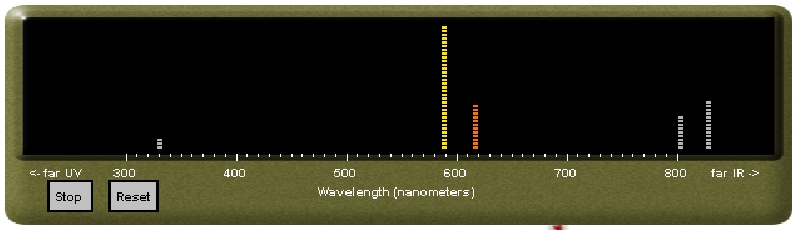
\includegraphics[width=0.5\linewidth]{3.png}}
   \caption{Датчик робота LiDAR; Кредити на зображення: Оптичний датчик дальності Garmin LIDAR-Lite (CC BY-NC-SA 2.0) від Adafruit}
 \end{figure}



\section{Які датчики використовуються у роботах?}\par

\subsection{Типи датчиків зору, що використовуються у робототехніці | Візуальні датчики }
Датчики зору використовують зображення для оцінки присутності, орієнтації та точності найближчих об'єктів. Отримання та обробка зображень поєднані у відеодатчиках, і багатоточковий контроль може виконуватися лише з одним датчиком. Обмін даними між відеокамерою та комп'ютерним процесором також здійснюється через датчики технічного зору. Монохромний та кольоровий відеодатчики – це дві форми відеодатчиків.

Камери необхідні роботам для переміщення по навколишньому середовищу та запобігання зіткненням з прилеглими об'єктами, оскільки вони є датчиками, які збирають та аналізують дані. 2D-зображення, 3D-зондування, ультразвукові та інфрачервоні зображення – все це приклади технологій камери.

\begin{figure}[h!]
   \center{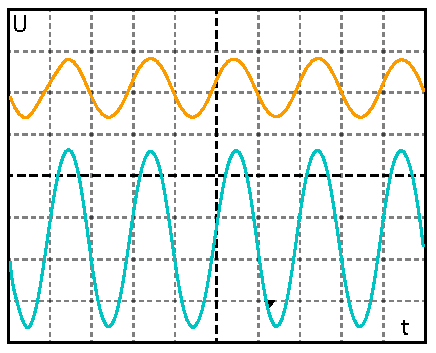
\includegraphics[width=0.8\linewidth]{4.png}}
   \caption{  Gisling, Робот Люфтваффен Ейгентум, CC BY-SA 4.0}
 \end{figure}

\subsection{2D Imaging}
Цифрові фотоапарати зовні нагадують плівкові, але в їхній основі лежать зовсім інші наукові концепції. Цифрова камера, на відміну від телевізора, яка створює зображення за пікселями, вловлює фотони і перетворює їх на електричний сигнал, який можна обробляти як число. ПЗЗ та КМОП – це два типи двовимірних цифрових фотоапаратів.

\subsection{3D зондування}
3D-зондування - ефективний інструмент для навігації роботів, оскільки він надає дані про обсяг, форму, місцезнаходження, орієнтацію та відстань об'єкта. Різні процеси, такі як стереозір, організоване світло та лазерна тріангуляція, можуть створювати тривимірні дані.

\subsection{Ультразвуковий}
Ультразвукові камери, також відомі як гідролокатори, розраховують проміжок часу між передачею та виявленням звукових хвиль, щоб визначити відстань між камерою та об'єктом. Інші ультразвукові датчики або роботи з ультразвуковими датчиками можуть бути виявлені за допомогою ультразвукових камер.
\begin{figure}[h!]
   \center{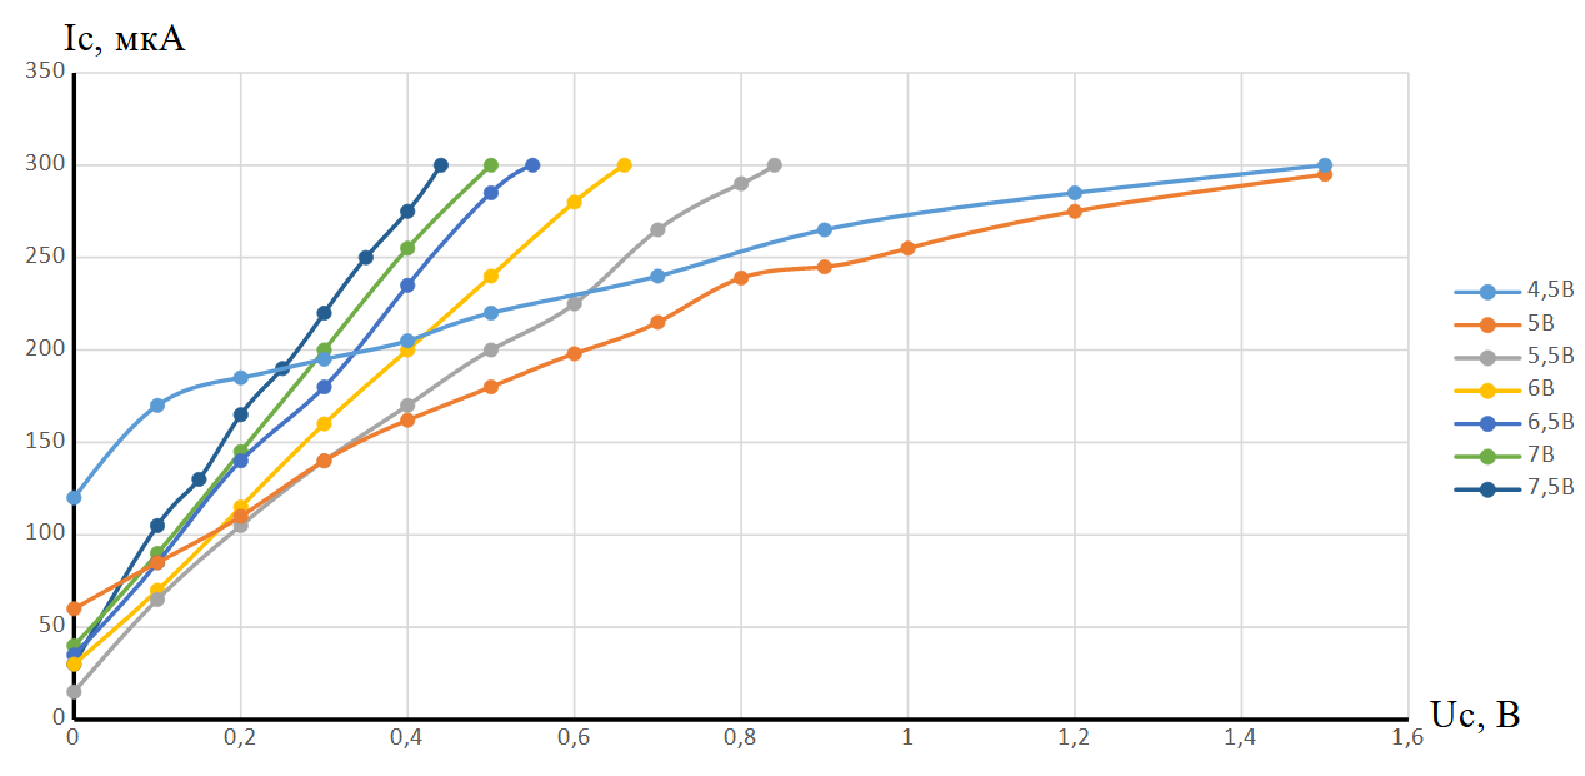
\includegraphics[width=0.8\linewidth]{5.png}}
   \caption{ Ультразвуковий датчик робота;   ведмідь від Pixabay}
 \end{figure}


\subsection{Робот з інфрачервоним датчиком}
Інфрачервоні датчики роботів виявляють інфрачервоні (ІЧ) промені, що випускаються об'єктом. Вони також можуть використовувати інфрачервоне світло для проектування на цільовий об'єкт і отримання відбитого світла для визначення його відстані або близькості. Інфрачервоні датчики економічні та можуть відстежувати інфрачервоне світло на великій площі. Вони також працюють у режимі реального часу. Вони краще, ніж ультразвукові датчики, описують краї об'єкта та відрізняють одне від одного.

\subsection{ІЧ-датчик, що працює в роботі-повідомнику лінії}
\begin{figure}[h!]
   \center{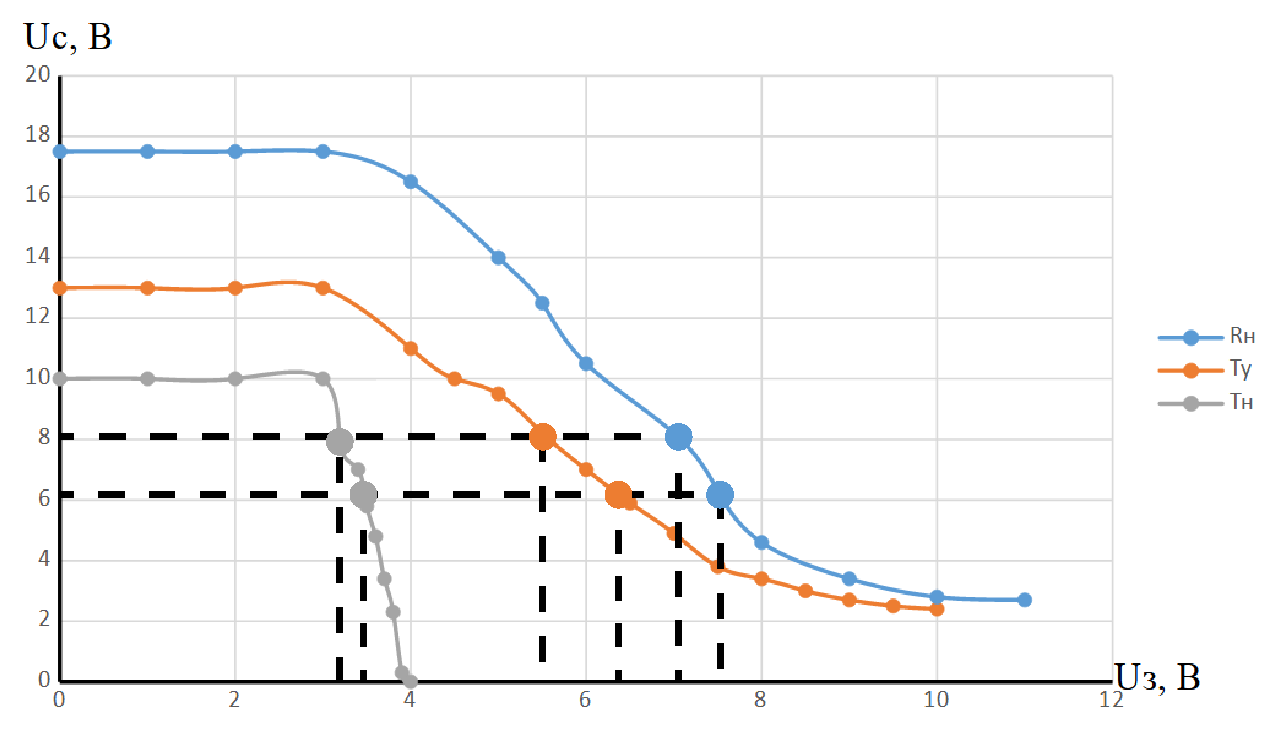
\includegraphics[width=0.8\linewidth]{6.png}}
   \caption{Marcmccomb, Послідовник лінії, CC BY-SA 3.0}
 \end{figure}


\section{Датчики навігації роботів}\par

У візуальній або оптичній навігації алгоритм комп'ютерного зору та оптичні датчики роботів, такі як лазерні далекоміри та фотометричні камери з матрицями ПЗЗ, використовуються для отримання візуальних характеристик, необхідних для локалізації в навколишньому світі, хоча є інші різновиди систем навігації на основі зору та методів локалізації. Нижче наведено важливі компоненти кожного методу:

\begin{itemize}
\item Уявлення про світ природи
\item Моделі для зондування
\item Алгоритми локалізації
\end{itemize}


Найпростіший спосіб змусити робота вирушити у певне місце – просто направити його. Це можна зробити різними способами, у тому числі закопати індуктивну петлю або магніти в підлозі, намалювати лінії на підлозі або вставити маяки, маркери або штрих-коди у навколишнє середовище. У промислових сценаріях такі автоматизовані транспортні засоби (AGV) використовуються для транспортних завдань. Роботи можуть переміщатися в приміщенні за допомогою систем внутрішнього позиціонування IMU.\\ 

Також було розроблено гідроакустичні навігаційні системи. Роботи також можуть використовувати радіонавігацію для визначення свого розташування. Бортовий польотний контролер використовує GPS для навігації та стабілізації, а супутникові системи функціонального доповнення (SBAS) та датчики висоти, такі як датчики атмосферного тиску, часто використовуються для вимірювання, а інерційні датчики використовуються в деяких бортових навігаційних системах роботів. Системи підводного акустичного позиціонування можуть керувати автономними підводними апаратами.

\section{Датчики сили у робототехніці}\par

  \subsection{Датчик сили руки робота}
  Датчики сили використовуються для визначення сил між основою датчика та чутливим шаром. Датчики FT, або датчики сили-моменту, сприймають як сили, так і моменти, що крутять. Зазвичай вони встановлюються безпосередньо перед робочим органом на руку робота. Датчики можуть використовуватися в широкому діапазоні додатків, і є недорогі аналогові датчики тиску до найпопулярніших 6-осьових датчиків FT.\\ 

  Оскільки вони є тактильними датчиками, їх можна використовувати визначення сили ковзання. Проте їх можна використовуватиме визначення потужності. Враховуючи різноманітність доступних датчиків сили, як зазначено нижче, може бути складно вирішити, який вам потрібен.\\ 
  \begin{enumerate}
  \item Простий датчик тиску.
  \item П'єзоелектричний датчик.
  \item Датчик на основі тензодатчика.
  \item Ємнісні FT-датчики.
  \item Ємнісні та резистивні гнучкі датчики сили.
  \end{enumerate}

\section{Датчик температури в робототехніці}\par
Датчики температури використовуються для виявлення змін температури навколишнього середовища, і це засновано на ідеї, що зміна напруги матиме те ж значення температури, що й навколишнє для зміни температури. TMP35, TMP37, LM34, LM35 та інші – одні з найбільш часто використовуваних ІС датчиків температури.

\section{Які датчики є у промислового робота?}\par

Двовимірні візуальні датчики, тривимірні візуальні датчики, датчик сили або моменту, що крутить, і датчики виявлення зіткнень є найбільш широко використовуваними датчиками для промислових роботів. Деякі  пояснюються так:

  \subsection{2D датчик технічного зору}
Двовимірний датчик зору - це камера, яка, крім іншого, може відстежувати об'єкти, що рухаються, і визначати їх місцезнаходження на конвеєрній стрічці. Це дозволяє виявляти та допомагати роботу у визначенні їхнього розташування, а потім робот може відповідним чином змінювати свій рух на основі отриманої інформації.

  \subsection{3D датчик технічного зору}
Щоб відчути третій вимір об'єкта, пристрій 3D Vision повинен мати дві камери або лазерні сканери під різними кутами. Наприклад, для вибору та розміщення деталей потрібне використання технології 3D Vision для ідентифікації об'єктів та створення 3D-зображень, а також для аналізу та вибору найкращого процесу вибору.

  \subsection{Датчик сил | Датчики крутного моменту в робототехніці}
Якщо візуальний датчик забезпечує робота очима, датчик сили/крутного моменту забезпечує роботу дотик. Сила кінцевого ефектора сприймається роботом за допомогою датчиків сили/крутного моменту. У більшості випадків датчик сили/крутного моменту розміщується між роботом та пристроєм, що дозволяє роботу відстежувати всі сили, що повертаються до пристосування.

  \subsection{Датчик виявлення зіткнення}
Цей датчик доступний у різних формах та розмірах, і його основна мета – забезпечити безпечне робоче середовище для операторів, які найбільше потрібні спільним роботам.

\section{Які датчики мають допоміжні роботи?}\par

Допоміжний робот - це комп'ютер, який може відчувати, обробляти та виконувати дії у повсякденному житті людей з обмеженими можливостями та людей похилого віку. Найпопулярнішим застосуванням датчиків роботів є використання ультразвукового сонара для допомоги сліпим. Протягом багатьох років роботи використовували ультразвукові гідролокатори як систему позиціонування.

\section{Датчик дальності у робототехніці | Робот із датчиком наближення}\par

Датчики дальності використовуються визначення відстані між об'єктом і стороною робота. Його робочий діапазон обмежений. Для розрахунку відстані використовують візуальну обробку. Роботи використовують датчики дальності, щоб переміщатися та уникати перешкод на своєму шляху. Спеціальні програми для датчиків діапазону повинні визначати положення та загальні характеристики форми компонента у робочій зоні робота. Джерелом освітлення у цих ситуаціях може бути джерело світла, лазерний промінь чи ультразвук.

\section{Датчики положення у робототехніці}\par

Будь-який датчик, який вимірює розташування об'єкта для використання в програмах управління, називається датчиком положення. Вони мають широкий спектр датчиків і безліч застосувань, від робототехніки до апаратів МРТ. Це один із найпотужніших датчиків, який використовується практично в кожному автономному транспортному засобі, що рухається.\\

Як обертальний, так і лінійний рух можна вимірювати за допомогою датчиків положення. Їх можна використовувати для обчислення абсолютного або відносного розташування. Безщіткові двигуни управляються поворотними датчиками, які часто відстежують кутові області різних механічних пристроїв у системі. Моторні енкодери - це датчики, що використовуються в робототехніці для відстеження розташування на круглому диску, перетворюючи положення в електричні імпульси, які можуть використовувати об'єкт контролю.

 \subsection{Управління становищем руки робота}
Шість окремих серводвигунів здатні переміщати кожне з'єднання у типовому шестиосьовому роботі. Енкодер двигуна використовується на задній стороні цих серводвигунів для підтримки положення. Щоб відстежувати обертання, вироблені серводвигуном, енкодер двигуна використовує вирізи в диску. Ці вимикачі виробляють світлові імпульси, які потім перетворюються на електричні імпульси.

 \subsection{Оптичний датчик положення у робототехніці}
Оптичні датчики використовуються для відстеження, підрахунку та позиціонування деталей без будь-яких дотиків. Доступні внутрішні чи зовнішні оптичні датчики. Внутрішні датчики зазвичай використовуються для вимірювання вигинів та інших незначних змін напрямку, тоді як зовнішні датчики збирають і передають певну кількість світла.

\section{Датчики швидкості у робототехніці}\par

Датчик швидкості або швидкості виконує кілька вимірювань положення через рівні проміжки часу та обчислює швидкість зміни значень положення з часом. Одним із основних датчиків швидкості, що використовуються в робототехніці, є тахометр.

 \subsection{Тахометр}
Тахометр - один з найважливіших пристроїв для забезпечення зворотного зв'язку за швидкістю. Він також використовується як лічильник оборотів та датчик оборотів. У двигуні тахометр використовується для вимірювання швидкості обертання валу. В аналоговому пристрої вихідний сигнал відображається у вигляді обертів за хвилину (оборотів за хвилину).


\section{Датчики прискорення у робототехніці}\par

Прискорення та нахил вимірюються за допомогою датчика прискорення пристрою, яке вимірює прискорення, відомого як акселерометр. Статична сила та динамічна сила - це два типи сил, які впливають на акселерометр.\\

-- Статична сила -- це сила тертя, що існує між двома речами. Ми можемо визначити, наскільки робот нахиляється, обчисливши силу тяжкості. Цей розрахунок допомагає збалансувати робота або вирішити, чи він рухається в гору або по плоскій поверхні.\\ 

-- Динамічна сила --  це стосується кількості сили, яка потрібна на переміщення об'єкта. Швидкість/швидкість робота можна визначити шляхом вимірювання динамічної сили за допомогою акселерометра.

\section{Датчики для роботів-пилососів}\par

Роботи-пилососи використовують різні датчики для виявлення перешкод та відстеження їх прогресу, а також для відкриття нових областей для дослідження, і ці датчики роботів-пилососів запускають запрограмовані реакції, які визначають, як робот повинен реагувати, якщо він зіткнеться з деякими перешкодами.


\begin{figure}[h!]
   \center{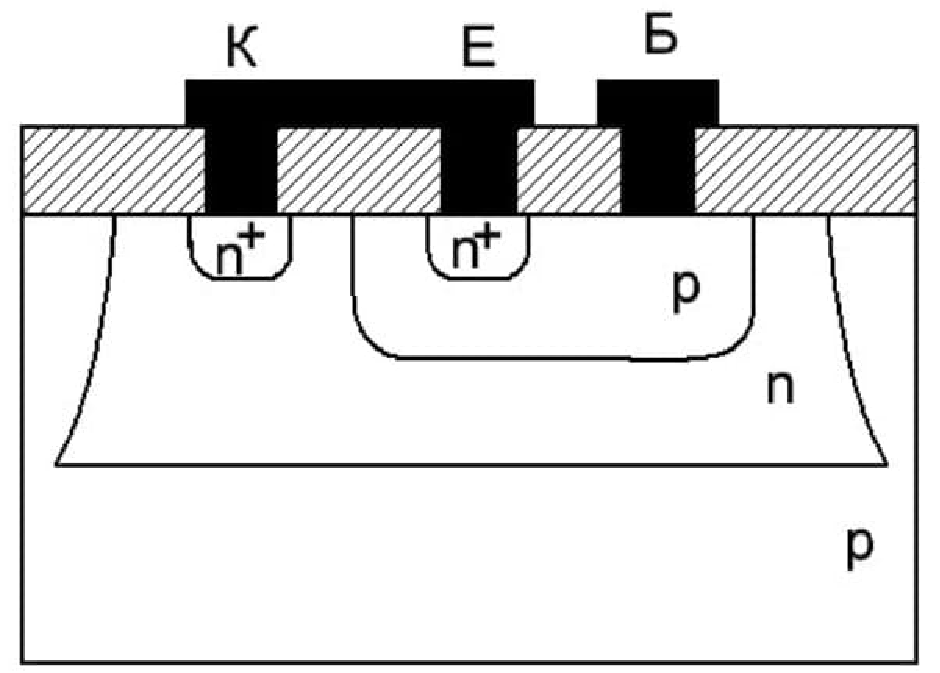
\includegraphics[width=0.7\linewidth]{7.png}}
   \caption{Робот-пилосос: PicaBot; Handitec, PicaBot Elite із технологією ActiveMapping, CC BY-SA 4.0}
 \end{figure}

 \subsection{Датчики перешкод}
Для роботи в домашніх умовах існують різні перешкоди, такі як ніжки стільців та столів, дивани, підставки для іншої побутової техніки, безпритульні іграшки тощо. вниз, і цей датчик буде активовано, коли бампер зіткнеться з перешкодою, і робот автоматично отримає команду розвернутися та піти.

 \subsection{Датчики обриву}
Сходи, мабуть, найнебезпечніша перешкода для роботів-пилососів; падіння може пошкодити вакуум, а також щось на своєму шляху. В результаті всі роботи-пилососи повинні мати датчики обриву як захід безпеки. Вони використовують інфрачервоні сигнали безперервного розрахунку відстані до поверхні підлоги.

 \subsection{Настінні датчик}
Вони фактично допомагають їм виявляти стіни за допомогою інфрачервоного світла, щоб вони могли йти за ними. Це дозволяє їм очищати краї стіни там, де вона зустрічається із підлогою. Найприємніше те, що вони можуть робити це, не дряпаючи стіну, як ми іноді робимо зі стоячими пилососами.

 \subsection{Колісні датчики}
Обертання колеса робота-пилососа вимірюється за допомогою світлових датчиків. Він оцінить, як далеко він проїхав, використовуючи це число та довжину кола колеса.


\section{Датчики, що використовуються в роботизованому зварюванні}




\subsection{Sensor Fusion Robotics}
У багатьох галузях та середовищах спостерігається зростання попиту на жорстких багатоцільових роботів, які є простими в установці. Тепер роботам необхідні сенсори для розуміння контексту та інтуїтивно зрозумілі інтерфейси для простоти використання. Деякі програми, наприклад, можуть використовувати розпізнавання жестів для керування фізичним пристроєм.

У той же час захист IoT, низьке енергоспоживання, безпека та надійність – все це суворі вимоги. Це часто спричиняє використання датчиків для контролю електричного струму, температури та інших змінних, щоб гарантувати, що система працює ефективно та безпечно. У найближчому майбутньому робототехніка збільшить кількість двигунів та універсальність довкілля, і в усьому світі з'явиться більше спільних роботів. Кількість датчиків, що використовуються роботами, збільшуватиметься в міру розробки більшої кількості систем керування та налаштувань.

























\begin{thebibliography}{9}
\bibitem{lit1} \href{http://www.kdpu-nt.gov.ua/sites/default/files/work_files/referat_signed.pdf}{: Р. В. Верба, В. О. Голуб, Г. М. Каказей, Г. А. Мелков,
О. О. Серга, О. І. Товстолиткін, А. В. Чумак, Д. Д. Шека. “Фізичні принципи спін-хвильової електроніки та спінтроніки” 2021p. }

\bibitem{lit2} <<Quantum Spin-Wave Materials, Interface Effects and Functional Devices for Information Applications>>
Jiapeng Xu, Lichuan Jin, Zhimin Liao, Qi Wang, Xiaoli Tang, Zhiyong Zhong1 and Huaiwu Zhang

\bibitem{lit3} Albisetti, E., Petti, D., Pancaldi, M., Madami, M., Tacchi, S., Curtis, J., et al. (2016).
Nanopatterning reconfigurable magnetic landscapes via thermally assisted scanning
probe lithography. Nat. Nanotechnol. 11 (6), 545.



 
\end{thebibliography}
\end{document}
